\chapter*{Workshop 2: One application, four environments}\label{workshop-02}
\addcontentsline{toc}{chapter}{W2: One application, four environments}

\section{Hold the task constant}

Run \texttt{npm run checkpoint -- 02}. Every presentation receives the same fixture: compilation succeeded, tests failed with an explanation, and publication is forty percent complete. Changing a presentation must not change those facts. The following specimens come from the companion's actual formatter and Bijou 7.2.0; they use Recursive Mono for the terminal cell projection. They are complete fixture outputs wrapped at forty cells for print. The interactive specimen shows presentation content; input routing and the runtime viewport are introduced in Workshop 3.

\subsection{Interactive and static}

\begin{minipage}[t]{.48\linewidth}
{\headingfont\large Interactive\par}\smallskip
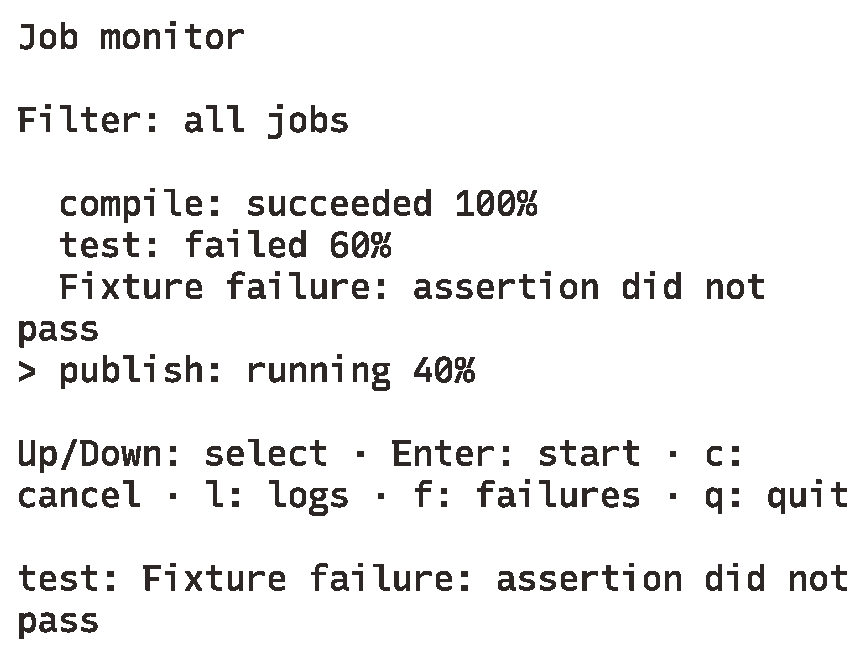
\includegraphics[width=\linewidth]{figures/monitor/monitor-interactive.pdf}
\end{minipage}\hfill
\begin{minipage}[t]{.48\linewidth}
{\headingfont\large Static / CI\par}\smallskip
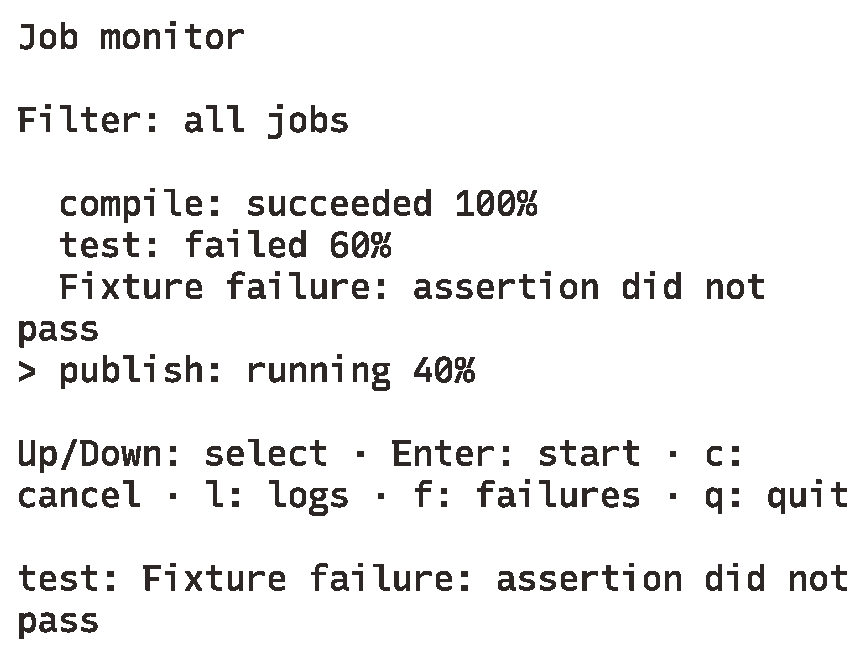
\includegraphics[width=\linewidth]{figures/monitor/monitor-static.pdf}
\end{minipage}

The rich mode provides an application loop in a terminal. Static mode emits a snapshot suitable for a CI log or a saved report. The two narrow specimens deliberately share a compact textual layout. The important difference is the delivery contract: a static invocation writes once and exits; an interactive invocation accepts input and redraws a viewport.

\subsection{Pipe and accessible}

\begin{minipage}[t]{.48\linewidth}
{\headingfont\large Pipe\par}\smallskip
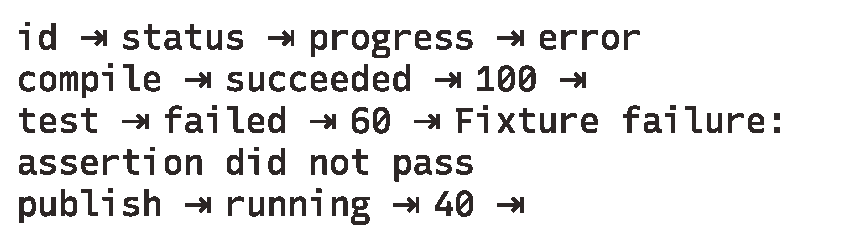
\includegraphics[width=\linewidth]{figures/monitor/monitor-pipe.pdf}
\end{minipage}\hfill
\begin{minipage}[t]{.48\linewidth}
{\headingfont\large Accessible\par}\smallskip
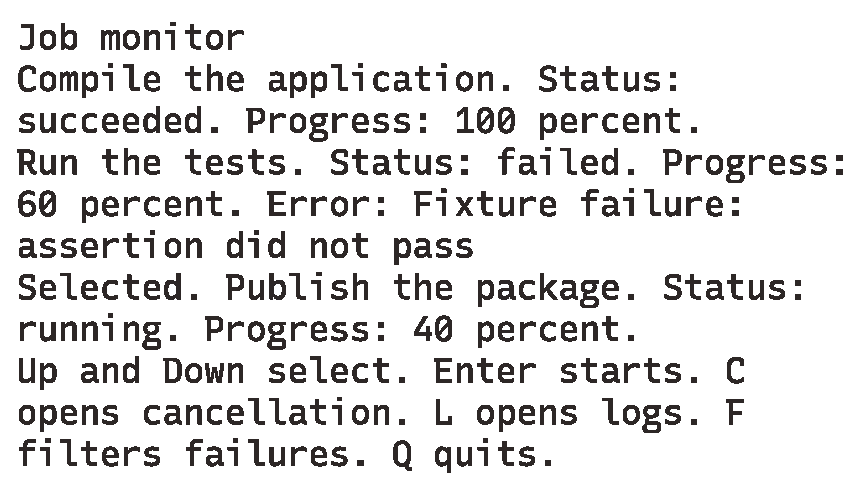
\includegraphics[width=\linewidth]{figures/monitor/monitor-accessible.pdf}
\end{minipage}

The pipe specimen makes tab characters visible as \texttt{⇥} for print. Its original TSV output is retained with the capture. It has stable identifiers, textual statuses, numeric progress and a separate error field. It has no cursor controls, decorative frame or keyboard help. The accessible presentation spells out selection, state, progress and the available actions. That is an explicit alternative presentation, not a claim that an automated text check establishes usability with every screen reader.

\section{Degrade honestly}

\subsection{Preserve the answer, choose the form}

A narrow terminal may replace a multi-column table with one compact record per job. A pipe should replace visual relationships with a stable serialization. An accessible view should state a selected relationship that a highlighted row might otherwise imply. In each case, ask what the reader still needs to understand and accomplish. The invariant is the task's useful meaning.

\subsection{Choose mode and styling separately}

The companion uses an explicit \texttt{--mode} choice when provided. Otherwise, redirected output chooses pipe mode; a CI environment attached to a TTY chooses static mode; an ordinary TTY chooses interactive mode. \texttt{NO\_COLOR} controls styling. It is not an instruction to erase interaction or replace a record format. These are application decisions made around the pinned Bijou API, not an assumption that every historical release detected modes in the same way.

For exact TSV without npm's script banner, use \texttt{node --import tsx src/main.ts --mode=pipe > jobs.tsv}, or npm's silent form documented in the companion. Inspect the saved file with a tab-aware tool. A terminal screenshot cannot establish that a data stream has the right number of fields.

\section{Break meaning before repairing style}

Run \texttt{npm run exercise -- color}. It fails because a colored dot is the only failure indication. Remove the color and the assertion has nothing useful to read. Diagnose the missing fact, then run with \texttt{--repair}. The repair uses a textual status. Color can reinforce that word later. Its cost is a less compact display; its benefit is that failure survives monochrome output, copying and speech.
